\section{Experimental Results}
\label{sec:results}

In this section, we first describe our test methodology and then present the results. Our experiments were configured as follows. We generated 30 VNFPP instances for each problem size and topology by varying the number and length of services and the size and speed of the VNFs. We assigned each algorithm a budget of 16000 evaluations to be used across all threads. All tests were run on a 8 core/16 thread CPU at 2.6GHz. All parallel algorithms were implemented using the parallelisation library Rayon.\footnote[1]{\url{https://github.com/rayon-rs/rayon}}

We used the parameter settings for NSGA-II proposed in \cite{DebAPM00} for NSGA-II, MD-NSGA-II and MS-NSGA-II. As PPLS/D is known to be sensitive to the population size \cite{ShiZS20}, we also consider a range of population sizes for each test. 

For analysis, we recorded the time each algorithm took to complete and the hypervolume of the final population. Since the three objectives typically have orders of magnitude different values it is necessary to first normalize the objectives. The utopian and nadir points were estimated by taking the best and worst objective values respectively from all tests. We used the reference point $1 + \epsilon$ for each objective where $\epsilon$ is a small number.

\begin{figure}[t]
    \begin{minipage}{\textwidth}
        \hspace*{-2.1em}
        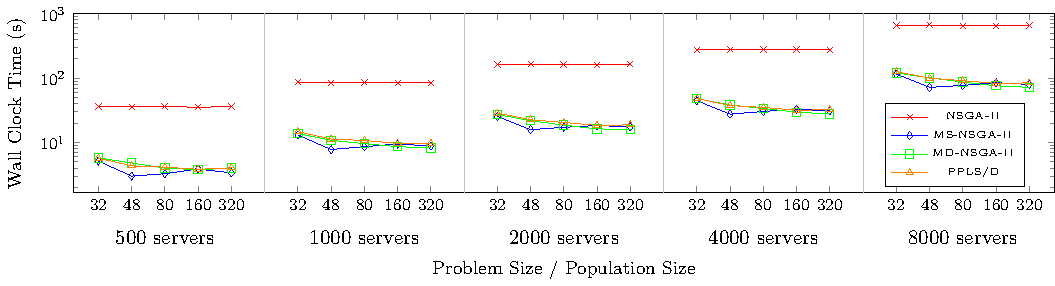
\includegraphics[width=1.05\textwidth]{figures/graphs/fat_tree_timing}
        \subcaption{Fat Tree}
        \vspace{1em}

        \label{fig:ft_tm}
    \end{minipage}

    \begin{minipage}{\textwidth}
        \hspace*{-2.1em}
        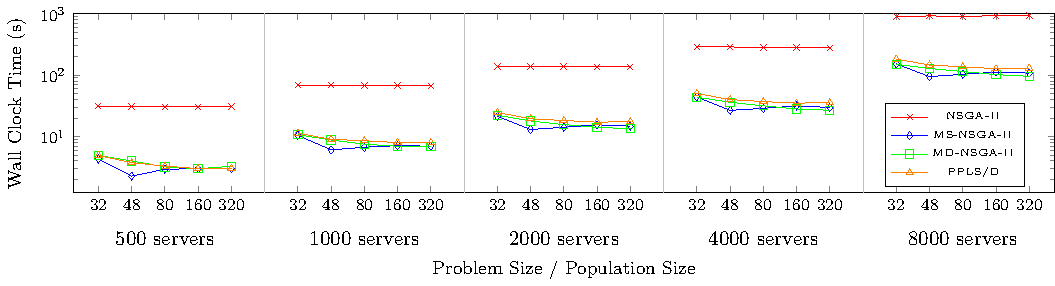
\includegraphics[width=1.05\textwidth]{figures/graphs/dcell_timing}
        \subcaption{DCell}
        \vspace{1em}

        \label{fig:dc_tm}
    \end{minipage}

    \begin{minipage}{\textwidth}
        \hspace*{-2.1em}
        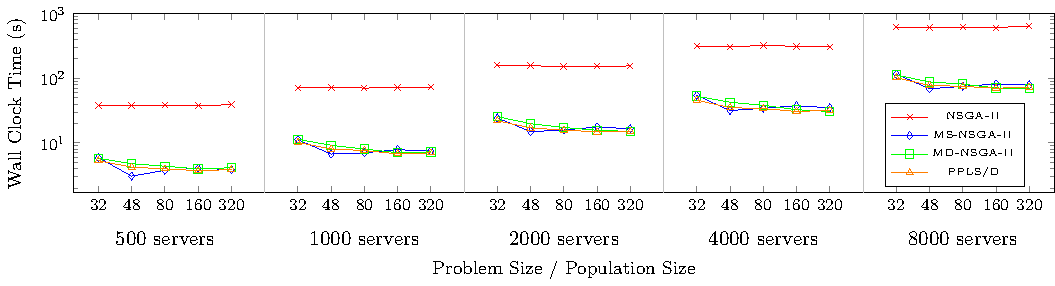
\includegraphics[width=1.05\textwidth]{figures/graphs/leaf_spine_timing}
        \subcaption{Leaf-Spine}
        \vspace{1em}

        \label{fig:ls_tm}
    \end{minipage}

    \caption{Mean Execution Time vs Problem Size and Population Size}
    \label{fig:et}
\end{figure}

\begin{figure}[t]
    \begin{minipage}{\textwidth}
        \hspace*{-2.1em}
        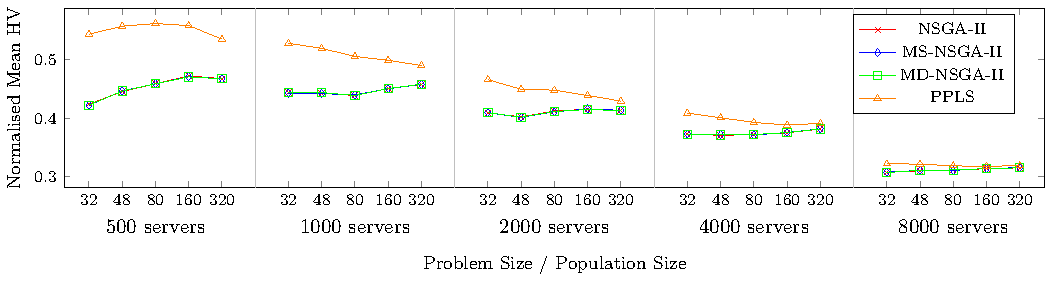
\includegraphics[width=1.05\textwidth]{figures/graphs/fat_tree_hv}
        \subcaption{Fat Tree}
        \vspace{1em}

        \label{fig:ft_hv}
    \end{minipage}

    \begin{minipage}{\textwidth}
        \hspace*{-2.1em}
        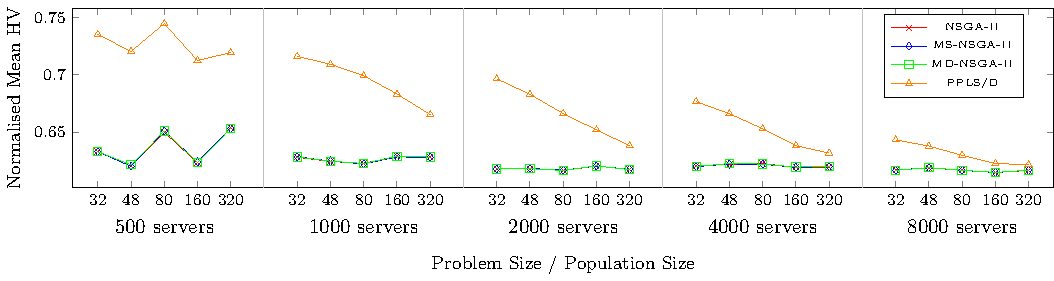
\includegraphics[width=1.05\textwidth]{figures/graphs/dcell_hv}
        \subcaption{DCell}
        \vspace{1em}

        \label{fig:dc_hv}
    \end{minipage}

    \begin{minipage}{\textwidth}
        \hspace*{-2.1em}
        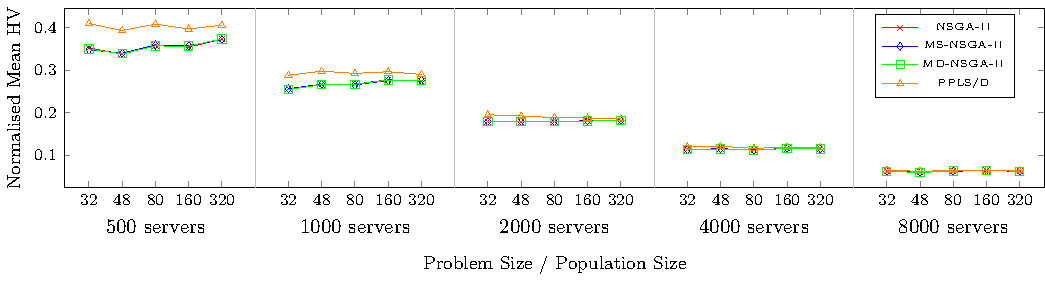
\includegraphics[width=1.05\textwidth]{figures/graphs/leaf_spine_hv}
        \subcaption{Leaf-Spine}
        \vspace{1em}

        \label{fig:ls_hv}
    \end{minipage}

    \caption{Mean HV vs Problem Size and Population Size}
    \label{fig:hv}
\end{figure}

Fig. \ref{fig:et} and Fig. \ref{fig:hv} demonstrate our two key findings. First, Fig. \ref{fig:et} shows that PMOEAs are typically 5-10x faster than the sequential NSGA-II. As the problem size increases, the time required to evaluate a solution also increases. However, this step can be parallelized reducing the overall execution time.

Second, Fig. \ref{fig:hv} shows that the speed improvements from parallelisation did not come at the cost of solution quality. This demonstrates that PMOEAs solve VNFPPs faster and at no cost to solution quality.

Further, when the best parameter settings are considered for each algorithm, PPLS/D found \textit{better} solutions on average than other algorithms on the majority of problems. These results must be considered with three caveats:

\begin{enumerate}
    \item PPLS/D was less effective on larger problem instances. Whilst all algorithms experienced some decline when solving larger problem instances, this behavior is particularly apparent with PPLS/D. PPLS/D relies on local search operators to explore the solution space. On large problem instances, the local search area is very large. It is likely that on large problems PPLS/D only explores the neighborhood of the initial population. Alternative local search operators may be able to explore the search space more effectively, however this remains for future research.

    \item PPLS/D is sensitive to the population size whereas the other algorithms were not. In the majority of instances, PPLS/D produced better sets of solutions when a small population was used. Shi et al \cite{ShiZS20} proposed this was due to large population sizes restricting each subproblem to a small region of the solution space. In PPLS/D, a subproblem can only consider a solution if it is the closest subproblem to the solution (see Section \ref{sec:algorithms}). With a large population, the solutions generated by the local search are more likely to be near to a different subproblem, reducing the number of solutions considered, and slowing the search process. This appears particularly important on larger problem instances wherein the setting of the population size was the most important factor in whether PPLS/D outperformed the other algorithms. 

    \item PPLS/D maintains an archive population and hence stores more solutions on the Pareto front than the other algorithms used. PPLS/D typically produced 1-2 orders of magnitude more non-dominated solutions than the other algorithms. This in part explains the improved hypervolume for PPLS/D as more solutions can better approximate the Pareto front.
\end{enumerate}

Despite these caveats, it is still notable that PPLS/D outperformed other algorithms using only local search operators. Some of the drawbacks of PPLS/D may be able to be resolved with alternative local search operators in future work.